
%% To submit your paper:
\documentclass[draft]{agujournal2019}
\usepackage{url} %this package should fix any errors with URLs in refs.
\usepackage{lineno}
\usepackage[inline]{trackchanges} %for better track changes. finalnew option will compile document with changes incorporated.
\usepackage{soul}
\linenumbers
%%%%%%%
% As of 2018 we recommend use of the TrackChanges package to mark revisions.
% The trackchanges package adds five new LaTeX commands:
%
%  \note[editor]{The note}
%  \annote[editor]{Text to annotate}{The note}
%  \add[editor]{Text to add}
%  \remove[editor]{Text to remove}
%  \change[editor]{Text to remove}{Text to add}
%
% complete documentation is here: http://trackchanges.sourceforge.net/
%%%%%%%

% \draftfalse

%% Enter journal name below.
%% Choose from this list of Journals:
%
% JGR: Atmospheres
% JGR: Biogeosciences
% JGR: Earth Surface
% JGR: Oceans
% JGR: Planets
% JGR: Solid Earth
% JGR: Space Physics
% Global Biogeochemical Cycles
% Geophysical Research Letters
% Paleoceanography and Paleoclimatology
% Radio Science
% Reviews of Geophysics
% Tectonics
% Space Weather
% Water Resources Research
% Geochemistry, Geophysics, Geosystems
% Journal of Advances in Modeling Earth Systems (JAMES)
% Earth's Future
% Earth and Space Science
% Geohealth
%
% ie, \journalname{Water Resources Research}

\journalname{JGR: Oceans}

\begin{document}
\section{Supplementary material}
\begin{figure}[ht!]
    \centering
    \includegraphics[width=1\linewidth]{figures/00_manuscript_supp_sst.png}
    \caption{Sea surface temperature (SST) in colors, obtained from the AVHRR dataset, gridded geostrophic currents from AVISO in gray vectors and cyclonic (blue) and anticyclonic (red) eddies from META3.4exp. On the left (a) a composite between 10th and 12nd March and on the right (b) a composite from 28th and 30th March. The black dots represents the vertical profiles selected in Figure 9.}
    \label{fig:supp_sst}
\end{figure}

\begin{figure}[ht!]
    \centering
    \includegraphics[width=1\linewidth]{figures/00_manuscript_supp_precip.png}
    \caption{Accumulated precipitation (in colors) from the MERGE dataset and the Ekman transport in black vectors. The conditions between 10th and 12nd March is presented in (a), between 13th and 16th March in (b) and 28th and 30th March in (c). The black dots represents the vertical profiles selected in Figure 9.}
    \label{fig:supp_precip}
\end{figure}

\begin{figure}[ht!]
    \centering
    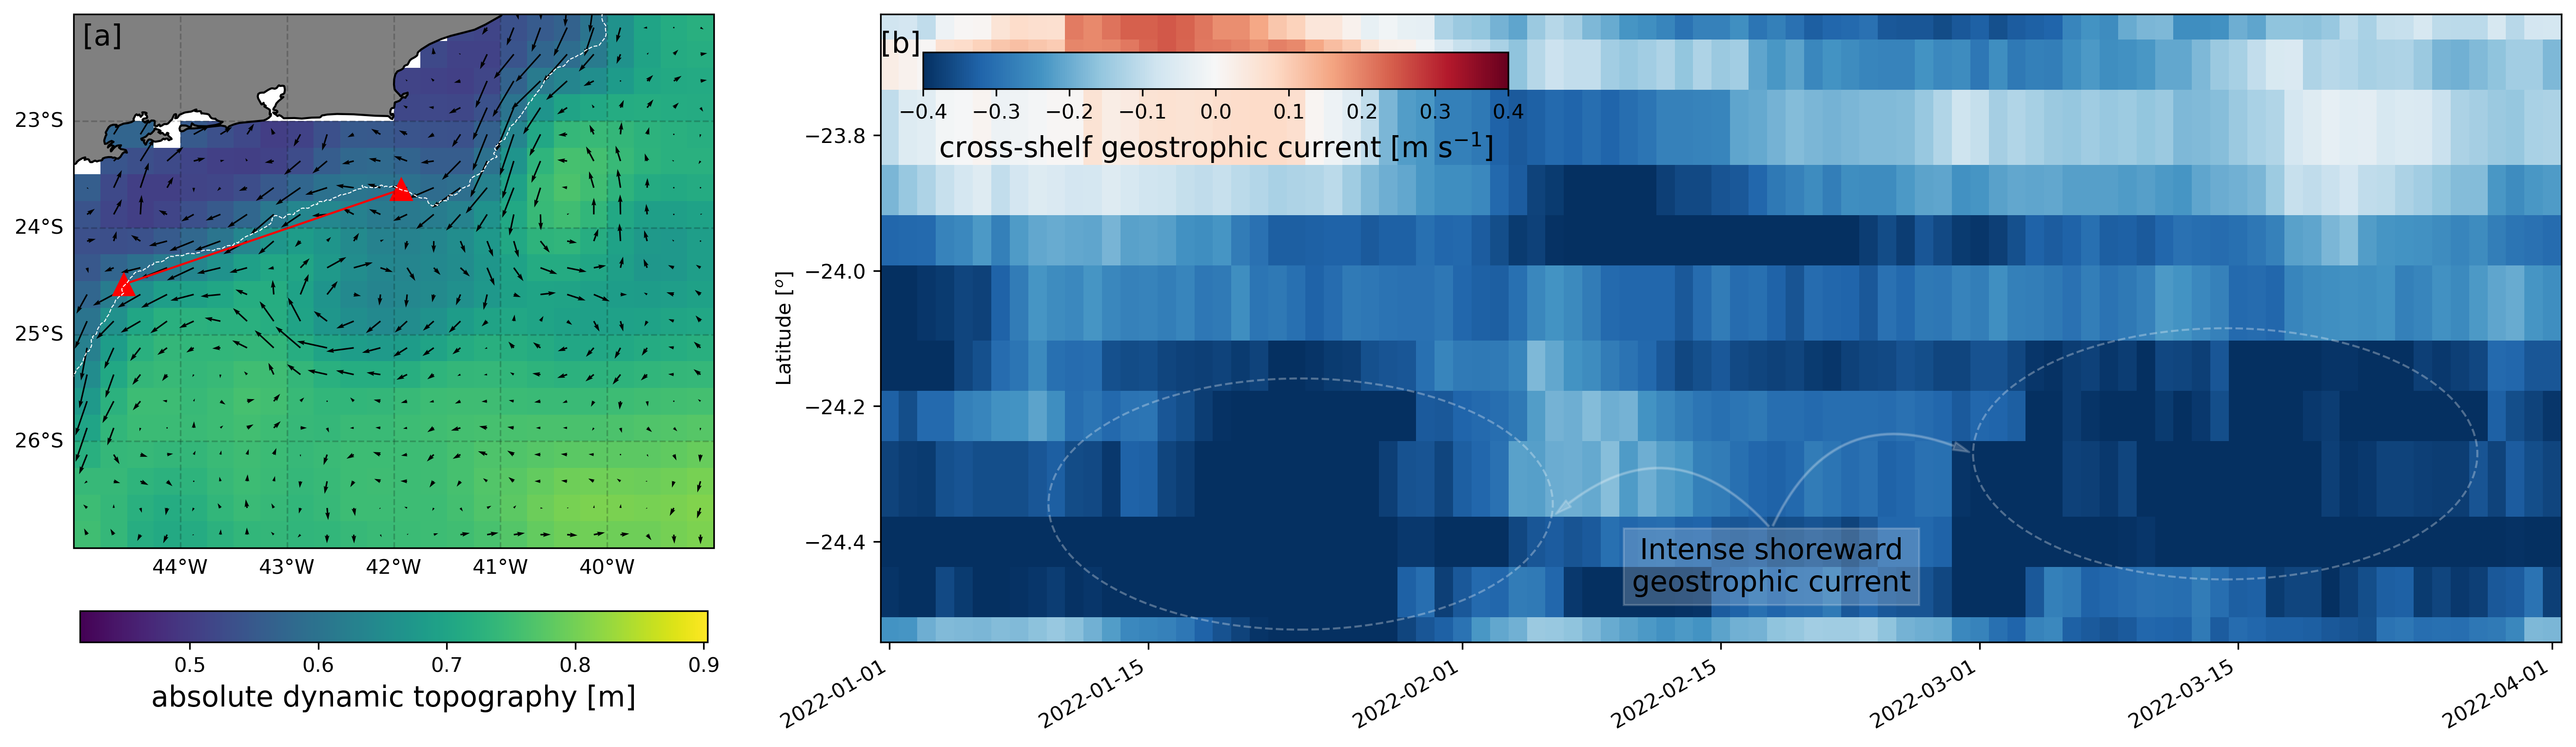
\includegraphics[width=1\linewidth]{manuscript/figures/00_manuscript_cross_geostrophic_new.png}
    \caption{Virtual along-shelf edge transect, red line on (a), with cross-shelf edge geostrophic velocities, in $m\ s^{-1}$. Blue (negative) values are shoreward and red (positive) offshoreward in (b).}
    \label{fig:cross_geostrophic}
\end{figure}
\end{document}